\section{Evaluation}
\label{sec:eval}

%\paragraph{Evaluation overview.}
Our evaluation answers the following questions.
(i) How well does {\sys} mitigate state-of-the-art network side-channel attacks?
%\mis{I woud be inclined to start with this.}
{(ii) What are the overheads associated with varying DP relevant
configuration parameters?}
%(ii) What are the theoretical bounds of differential privacy guara2.5 and the
%associated overheads in network side-channel mitigation?
(iii) What are the packet latency overheads and the peak line rate and
throughput sustained by our {\sys} middlebox?
(iv) What are {\sys}'s overall costs on privacy, bandwidth, client latency, and
server throughput for different classes of applications?
(v) How do {\sys}'s privacy guarantees and performance overheads compare to
prior techniques?

\if 0
(i) What are the trade-offs in the choice of various configuration parameters
that affect packet latencies, bandwidth overheads, and privacy guarantees?
(\Cref{subsec:privacy-microbenchmarks}
(ii) What are the optimal packet latencies, line rate, and number of concurrent
tunnels that can be supported by a MinesVPN middlebox?
(\Cref{subsec:perf-microbenchmarks})
(iii) Does MinesVPN mitigate network side-channel attacks in the applications?
(\Cref{subsec:attack-eval})
(iv) What are privacy guarantees, and the overheads on bandwidth, client latency
and server throughput due to {\sys}'s shaping on different classes of
applications---video and web?  (\Cref{subsec:eval-video,subsec:eval-web})
(v) How do {\sys}'s privacy guarantees and performance overheads compare to
prior techniques? (\Cref{subsec:eval-video,subsec:eval-web})
\fi
%(iii) What are the trade-offs between privacy guarantees and bandwidth overheads
%incurred for the applications?
%(v) What are the overheads on client response latencies and peak server
%throughput of the applications using MinesVPN?
%In the following subsections, we present (i) an empirical evaluation of the
%trade-offs between privacy leakage rate and the overheads incurred due to
%{\sys}'s differentially private shaping, (ii) microbenchmarks to analyze the
%overheads introduced due to {\sys}'s middleboxes, (iii) {\sys}'s impact on
%client latencies and server throughput in the context of our two applications,
%and (iv) an empirical evaluation of {\sys}'s security in the two applications.

%{\sys}'s middlebox components can run on top of a standard Linux kernel.
For our experiments, we use four AMD Ryzen 7 7700X desktops each with eight 4.5
GHz CPUs, 32 GB RAM, 1 TB storage, and one Marvell AQC113CS-B1-C 10Gbps NIC. We
simulate client and server applications on two of the desktops and {\sys}'s
middleboxes on the other two desktops.
The middleboxes are connected to each other via an additional Intel X550-T2
10Gbps NIC on each desktop.
%The middleboxes contain one additional Intel X550-T2 10Gbps NIC each and are
%connected to each other via these NICs.
The client and server desktops are connected to one of the two
middleboxes each via the Marvell NICs, overall forming a linear topology.

We implemented the {\ushaper} and {\dshaper} processes in
\update{1100} and \update{1800} lines of C++ code, respectively, and deployed
them on Ubuntu OS 22.04.02 (kernel version 5.19).
{\sys} relies on the MSQUIC implementation of QUIC, libmsquic v2.1.8, which
includes OpenSSL for traffic encryption, contributing an additional
\update{180713} LoC to {\sys}'s TCB.

For rapid evaluation, we  built a simulator,
which implements the {\prepare} thread's DP logic.
The simulator transforms  an application's original packet sequence (from
tcpdump) into a sequence of burst sizes within fixed-length
intervals, and outputs a sequence of transmit sizes corresponding to DP
queries.
%
{We confirmed that the bandwidth overheads from the simulator closely match
the overheads observed on the testbed. Thus, we report privacy and
bandwidth overhead results from the simulator and latency and
throughput results from the testbed, unless specified otherwise.}
%We implement {\sys}'s middlebox on a \todo{X} server with \todo{8} \todo{Intel
%XXX} CPUs, \todo{X} RAM, and \todo{two Intel XXX XGbps} NICs. We disable
%hyperthreading and dynamic voltage and frequency scaling (DVFS) on the servers
%mainly to reduce variance in the empirical measurements. We use two KVM virtual
%machines to host the network stacks of {\unshapedVM} and {\shapedVM}.  Each VM
%is configured with \todo{X vCPUs, X GB RAM and X GB storage} and is connected
%to one NIC each. Each VM's vCPUs are statically pinned to one physical core
%each. The VMs run on \todo{Ubunutu XXX and XXX kernel}. The {\shapedVM} runs
%the \todo{QUIC version XXX}~\cite{QUIC} on top of the kernel.
%

%In principle, {\sys} can support arbitrary protocol stacks on the end hosts.
%In our evaluation, we consider applications using TCP, which presents the most
%challenging protocol stack due to its own implementation of reliable delivery,
%congestion control, flow control, loss recovery, and retransmissions.
We use two applications for case studies, a video streaming service and a
medical web service, which we describe below. Both applications are hosted on an
Nginx 1.23.4 web server and the datasets are stored on the host file system.
%We evaluate {\sys}'s effectiveness in hiding from an adversary the time and
%content of clients' interactions with these services, and the bandwidth,
%latency, and throughput overheads incurred due to shaping.
%We briefly describe the services below.

\textbf{Video service.}
The video streaming service is used to serve \update{100 YouTube videos} in 720p
resolution with \update{5 min to 130.3 min (median 12.6 min)} durations and
\update{2.7 MB to 1.4 GB (median 73.7 MB)} sizes.
We implement a custom video streaming client in Python, which
uses one TCP connection for a single stream and requests individual 5s segments
from the service synchronously.
Unless specified otherwise, we stream the first 5 min of videos in our
experiments. The configuration is in line with that used in prior
work~\cite{schuster2017beautyburst} and reasonable, given the popularity of
short videos~\cite{videostats}.
%to fetch all segments of a single video~stream.

%We implemented a custom video streaming service in PHP, which is hosted using
%Apache HTTP Server \todo{XXX}, and returns video segments in response to client
%requests. We host \todo{1218} Youtube videos in 240p and 720p bitrates, which
%are generated using MPEG-DASH encoding. The videos have durations
%ranging from \todo{X min to 4.2 hours (median: 7 min)}, and with the
%video sizes ranging from \todo{X KB to 6.2 MB (median: 6.2 MB)}. \todo{TODO:
%comment on simulating a live streaming setup.}
%%
%We also implemented a custom client in Python, which first requests
%for the MPD segment of a video from the server, parses the MPD, and then
%requests for subsequent video segments sequentially.

\if 0
\paragraph{VoIP.}
\am{May go depending on the results. Replace with multi-tier web service
instead.}
We use FlexiSIP~\cite{flexisip} as a VoIP server and
Linphone~\cite{linphone} application as a client, both of which are hosted in
separate containers on Docker \todo{XXX version} inside a VM with \todo{Ubuntu
18.04 LTS and XXX kernel}. We use the DAPS dataset~\cite{daps} of \todo{X}
audio clips from \todo{source}~\cite{audio-dataset}. The audio clips are
encoded using \todo{G.722} and have durations ranging from \todo{X-Y min
(median: Z min)} and sizes ranging from \todo{X-Y KB (median: Z KB)}.
\fi

\textbf{Web service.}
The web service is used to serve a corpus of {96} static HTML pages of a medical
website, whose sizes range from \update{54 KB to 147 KB (median: 90 KB)}.
{As a client, we use modified wrk2 \cite{wrk2} that issues concurrent
asynchronous HTTPS GET requests at a specified rate.}

For all experiments, we use one baseline setup and one of three {\sys}
configurations.
In the baseline setup ({\base}), the client is directly connected to the server.
In the simulator setup ({\nssim}), we generated sequences of shaped burst sizes
using DP shaping.
With {\sys}, the traffic between the client and the server passes through two
middleboxes, each implementing {\ushaper} and {\dshaper}.
We consider two configurations of the middleboxes:
(i) {\nsnoshape}: {\dshaper} does not implement shaping (\ie neither DP noise
sampling nor the fixed length loop interval $\dpintvl_{max}$), allowing us to
measure the system overheads due to the middlebox implementation, and
(ii) {\ns}: {\dshaper} implements the full shaping mechanism.
{By default, each middlebox is configured with 128 pairs of per-flow
transmit and receive queues (unless specified otherwise). We configure the queue
sizes for the max data that can be transmitted at line rate for a given
DP shaping~interval. We configure a max cutoff for the shaped buffer length
based on the max burst length of the application and the number of active
flows. This implies that the number of flows is public.}
%each of length 12.5 MB (unless specified otherwise).}
% \ml{This mean that the total number of flow is public in \sys.}
% \ml{Point to the fix if we have it!}

In addition, we compare with two other shaping strategies: constant-rate shaping
({\constshape}), which is the most secure shaping strategy, and Pacer
({\pacer}), a SOTA system that shapes traffic on a per-request basis.
%We compare bandwidth overhead of {\sys} with the overheads~that would be
%incurred due to constant rate shaping ({\constshape}) and~Pacer
%\cite{mehta2022pacer} (\S\ref{subsec:eval-comparison}), a SOTA system that
%provides dynamic shaping on a per-client request basis.
%We also compare the accuracy of attacks on traffic shaped by {\sys}, constant
%rate shaping and Pacer (\S\ref{subsec:attack-eval}).
For {\constshape}, we configure the peak load corresponding to the largest
object sizes in our applications, which involves transmitting 1.7MB in 5s for
videos and 57KB in 50ms for web.
For Pacer, we pad all web pages to the largest page size, \ie 147KB in our
dataset. For videos, Pacer pads a segment at $i$\textsuperscript{th} index
in a video stream to the largest segment size at that index across all videos in
the dataset.


\begin{figure}[t]
    \centering
    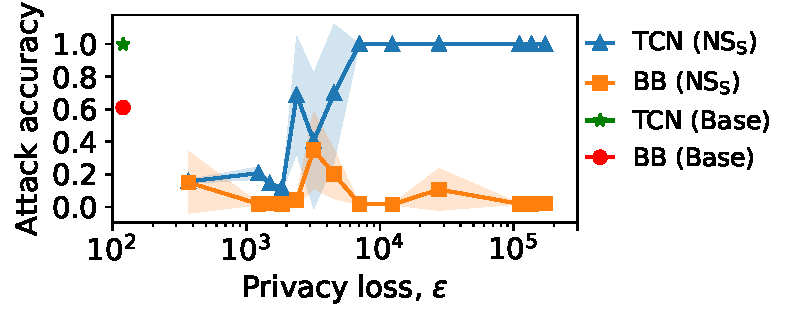
\includegraphics[width=0.85\columnwidth]{accuracy_vs_privacy_loss_video_updated.pdf}
    \caption{\update{Classifier accuracy on shaped traces.}
        %    \am{Change label from {\ns} to {\nssim}}
    }
    %\am{How is the blue shaded area going higher than accuracy of 1.0?}\as{The
        %blue shaded area is +-std so it can be larger than one or smaller than
        %zero.}
    \vspace{-0.4cm}
    \label{fig:empirical-privacy}
\end{figure}

\subsection{{\sys} Defeats Attack Classifiers}
\label{subsec:attack-eval}
%\todo{We need to explain that the accuracy of classifier on pacer and CR is as
%good as random guess (\ie 2.5\%)}.
%\\
%\am{Allude to formal proof of guarantees and security by design.}
%We measure the impact of the privacy configurations on the performance of
%attack classifiers \todo{from \S\ref{subsec:attack-bg}} on shaped traffic of
%video streams.
We start with an empirical evaluation of the privacy offered by {\sys}'s traffic
shaping. Recall that the traffic shaping depends on several DP parameters: the
window length $\winlen$, the sensitivity $\qsens$, the length of the DP
interval $\dpintvl$, and the privacy loss $\varepsilon$.
%We train the classifiers from
%\S\ref{subsec:attack-bg} on shaped video traffic generated with varying
%$\epsilon_w$ values and evaluate their accuracy.
%Furthermore, we identify the weakest privacy configuration that is able to
%successfully defeat the classifiers.
We evaluated the classifiers from \S\ref{subsec:attack-bg} on shaped traffic generated using various values of these DP relevant parameters.
We present the classifiers' performance based on~only one set of values for
$\winlen$, $\qsens$, and $\dpintvl$, while varying $\varepsilon$ between
\update{[200, 200000]}.
Our goal is to provide intuition about what values of $\varepsilon$ are
sufficient to thwart a side-channel~attack.
%We analyze the performance of the classifiers on network
%traces collected from the testbed in our local network.
%\todo{We collect tcpdump traces from the {\dshaper} process in both the
%middleboxes and apply the TCN and BB classifiers on the collected traces.
%Note that these traces present a best case for the adversary;
%in practice,
%%under the assumption that the adversary is not colocated with the application,
%(i) the adversary can only measure the traffic between the middleboxes, and (ii)
%real measurements likely have more noise due to interference from other traffic
%on the Internet.}

We set (i) $\winlen = 5s$ to align with the 5s video segments that comprise the
videos, (ii) \update{$\qsens = 2.5 MB$}, \update{which covers 99th \%ile}
of the distances in our dataset (\S\ref{sec:eval-extended}), and
(iii) $\dpintvl = 1s$, which
leads to composing the privacy loss over $\varnumupdates = 5$ DP queries on
the buffering queues. The 1s interval provides a reasonable trade-off between
privacy loss, and bandwidth and latency overheads, which we
discuss in the subsequent sections.
%We discuss the rationale behind the configuration choices in the subsequent
%sections.
%
%We~vary per-window privacy loss, $\varepsilon_\winlen$, between \update{[100,
%10000]}.

We used 40 videos of 5 min duration each. We streamed each video 100 times
through our testbed without shaping~and collected the resulting tcpdump
traces. For each value of \update{$\varepsilon$}, we transformed each unshaped
trace into a shaped trace using our simulator to generate a total of 4000
shaped traces.
%For {\constshape} we pad each video segment to 1.7 MB and transmit it in
%5s intervals. For Pacer, we group all videos into a single cluster and pad the
%$i$\textsuperscript{th} segment in each video to the largest segment size at
%that index across all videos in the dataset.
We also shaped traces for {\constshape} and {\pacer}.
%We then train the classifiers on the shaped traces using 80-20 train-test split,
%similar to \S\ref{subsec:attack-bg}.


%For shaping, we set $\ssens = 1MB$, $\winlen = 5s$, and perform DP
%queries at $\dpintvl = 1s$ intervals in each window.
%\mis{Why???}
%For shaping, we select (i) window length ($\winlen$) of 5s, because it aligns
%with the 5s video segments that make up the videos, (ii) sensitivity ($\ssens$)
%of 1 MB, which covers 97\% of the video streams in our dataset
%(\S\ref{sec:eval-extended}), and (iii) interval length ($\dpintvl$) of 1s,
%which
%leads to composing privacy loss over 5 DP queries of the buffering queues
%(i.e. $\varnumupdates = 5$).
%We~vary per-window privacy loss, $\varepsilon_\winlen$, between \update{[100,
%10000]} and, for each value of $\varepsilon_\winlen$, we collect \update{100}
%normalized traces each of the shaped traffic of \update{40} videos streamed for
%\update{5 min}.
%Classifier training is same as in \S\ref{subsec:attack-bg}.


\update{
We train and test BB and TCN on shaped traces as in \S\ref{subsec:attack-bg} and
report the average and standard deviation of the accuracy of each classifier
over three runs.
}
Recall from \S\ref{subsec:attack-bg}, the BB and TCN accuracy on unshaped
traffic ({\base}) is 0.61 and 0.99, respectively.
%generated using the above configurations.
%\mis{I think this would be more helpful if we could draw lines at the accuracy
%of each model on unshaped, but encrypted traffic. I found the explanation below
%confusing, but didn't want to try to rewrite it without seeing how well the
%models do on the encrypted but unshaped traffic. In my mind, the high level take
%away is that $epsilon_W$ of between $10^2$ and $10^3$ is sufficient to thwart a
%state of the art attack; given that, the results from the current 6.1 can now be
%put in context, because we can explain how much that costs in terms of
%overhead.}
\update{For {\constshape} and {\pacer}, the accuracy of both BB and TCN
classifiers is 0.025. This is expected since both strategies transform all
unshaped traces into a single shape.
}

\Cref{fig:empirical-privacy} shows the classifiers' performance with {\sys}.
%(markers show average, shaded region shows the standard deviation).
While BB does not perform well for nearly all values of \update{$\varepsilon$},
TCN can be thwarted for \update{$\varepsilon$} upto 1000.
%
%We should
%\todo{We get similar results even when generating shaped streams with $\dpintvl
%= 0.1s$.}
{\em While even \update{{$\varepsilon \approx 200$}} is too
large to offer meaningful theoretical privacy guarantees, it is sufficient to
defeat SOTA attacks.}
%\mis{This seems like a really important result or observation; I believe
%what we're saying here is that theoretical analsys suggests that you need
%quite strong privacy guarantees, but from a practical perspective, this
%applicaiton requires much weaker guarantees.  I think this has potentially
%significant consequences.}
%\Cref{subfig:high-sensitivity-epsilon-sigma} shows that $\varepsilon_{\winlen} =
%100$ yields a noise overhead of $< 1 MB$ per window.

%While BB does not perform well for nearly all values of $\varepsilon_{\winlen}$,
%TCN's accuracy is less than 0.2 and close to 1.0 for $\varepsilon_{\winlen} =
%100$ and $\varepsilon_{\winlen} > 1000$, respectively.
%and \Cref{tab:attack_performance} demonstrates the performance of the same
%classifiers on the unshaped traffic.
%
%From \Cref{subfig:high-sensitivity-epsilon-sensitivity}, $\varepsilon_{\winlen}
%= 100$ yields a noise overhead of $< 400KB$ per window.
%The results highlight {\em (i) the huge gap between the theoretical DP
%guarantees and the configurations required to defeat SOTA attacks, and (ii)
%the costs of privacy required in the face of more sophisticated attacks in the
%future.}

\begin{figure}[t]
    \centering
    \begin{subfigure}{0.49\columnwidth}
        \centering
        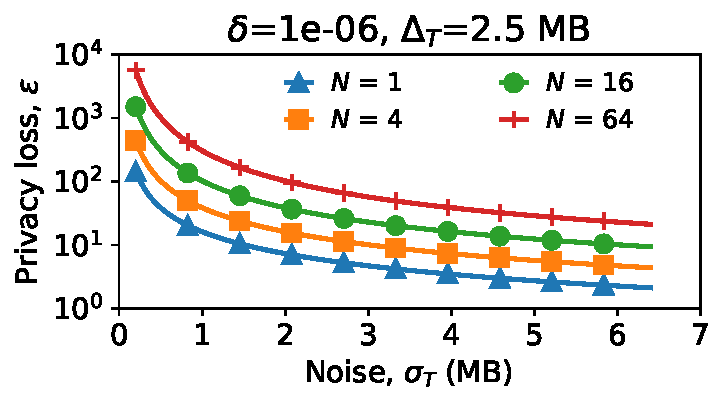
\includegraphics[width=\textwidth]{privacy_loss_VS_noise_std_video_updated.pdf}
        \caption{}
        %        \caption{Noise vs privacy loss}
        \label{subfig:high-sensitivity-epsilon-sigma}
    \end{subfigure}
    \hfill
%    \begin{subfigure}{0.33\textwidth}
    %        \centering
    %
    %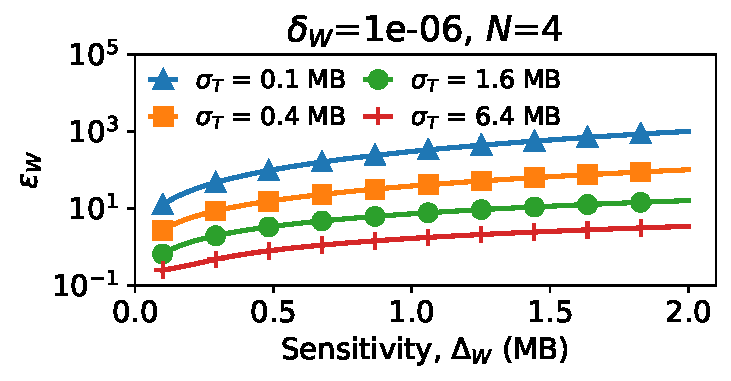
\includegraphics[width=\textwidth]{plots/privacy_loss_VS_sensitivity_video.pdf}
    %        \caption{Sensitivity vs privacy loss}
    %        \label{subfig:high-sensitivity-epsilon-sensitivity}
    %    \end{subfigure}
%    \hfill
    \begin{subfigure}{0.49\columnwidth}
        \centering
        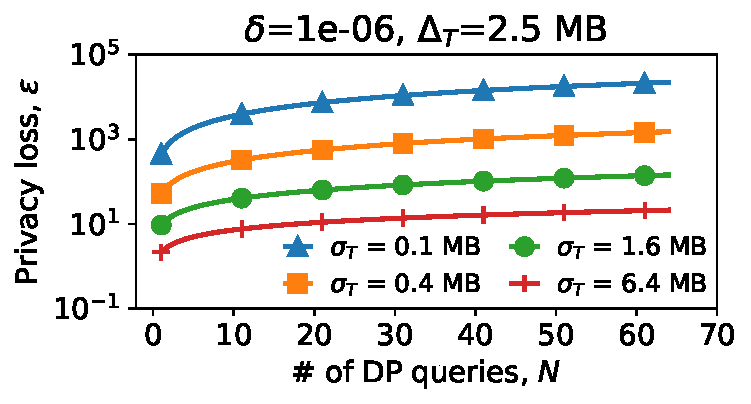
\includegraphics[width=\textwidth]{privacy_loss_VS_query_num_video_updated.pdf}
        \caption{}
%        \caption{\# of DP queries vs privacy loss}
        \label{subfig:high-sensitivity-epsilon-queries}
    \end{subfigure}
    \caption{
      \update{Privacy loss vs
      (a) noise and (b) \# of DP queries.}
%    \am{Make notations consistent.}
    }
    \vspace{-0.4cm}
    \label{fig:privacy-microbenchmarks}
\end{figure}


% \subsection{Theoretical Privacy Analysis}
\subsection{Impact of Privacy Parameters}
\label{subsec:privacy-microbenchmarks}

%We start by comparing the relation between DP relevant configuration parameters.
%Recall from \S\ref{sec:dp}, {\sys}'s privacy loss ($\varepsilon_\winlen$) and
%bandwidth overheads due to DP noise (represented by $\sigma_\dpintvl$, \ie the
%standard deviation of the noise distribution function) depend on:
%Recall from \S\ref{sec:dp} that {\sys} shapes traffic in uniform intervals of
%length $\dpintvl$, defined within a larger window of $\winlen$. Thus, {\sys}'s
%bandwidth overheads due to DP noise (denoted by $\sigma_\dpintvl$, \ie the
%standard deviation of the noise distribution) is measured in $\dpintvl$, while
%privacy loss ($\varepsilon_{\winlen}$) is defined in $\winlen$. These metrics
%depend on $\ssens$, $\delta_{\winlen}$, $\winlen$, and
%$\varnumupdates = \numupdates$.
%%Rather than exploring different values of $\winlen$ and $\dpintvl$, we
%%analyze $\varepsilon_{\winlen}$ and $\sigma_\winlen$ costs as a factor of
%%$\varnumupdates$.
%Given values for $\ssens$ and $\varnumupdates$, the
%$\varepsilon_{\winlen}$ and $\sigma_\dpintvl$ costs remain the same at
%different time scales.
%Thus, we explore $\varepsilon_{\winlen}$ and $\sigma_\dpintvl$ costs for
%different ranges of $\ssens$ and $\varnumupdates$, and analyze the impact of
%$\winlen$ and $\dpintvl$ on latency overheads separately.
%\ml{I don't get what these last few sentences mean? Is something like ``The
%core parameters influencing the behavior of the system are $\varnumupdates$
%and
%$\sigma_\dpintvl$. We thus explore their impact of the DP guarantee
%$\varepsilon_{\winlen}$. We analyse the impact of $\winlen$ and $\dpintvl$ on
%latency overheads separately.''?}
%A value of $x$ for $\varepsilon_\winlen$ implies that the probability of
%identifying the traffic content given a shape is $e^{x}$.
%The value of $\sigma_\winlen$ indicates the standard deviation of the noise
%distribution function, which estimates the amount of overhead that would be
%added to the original traffic due to DP shaping.
%All analyses use $\delta_\winlen = 10^{-6}$.
%which is a typical value in DP mechanisms.
%\mis{This could use a reference.}
%\ml{we could stick to ``All analyses use $\delta_\winlen = 10^{-6}$.'', it's a
%longer discussion and I don't know good citations...}
%At a high level, $\winlen$ affects $\ssens$, while $\ssens$,
%$\varepsilon_\winlen$, $\delta_{\winlen}$, and $\varnumupdates$

We now  evaluate how $\varepsilon$ varies with $\qsens$,
$\sigma_\dpintvl$, and $\varnumupdates$.
Due to space constraints, we present plots for a fixed value of $\qsens
= 2.5 MB$ and defer other plots to \S\ref{sec:eval-extended}.
All analyses use $\delta = 10^{-6}$.

\Cref{subfig:high-sensitivity-epsilon-sigma} shows the tradeoff between
$\varepsilon$ and $\sigma_\dpintvl$ over four different values of
$\varnumupdates$.
Intuitively, a larger
$\sigma_\dpintvl$ implies higher bandwidth overhead due to DP shaping.
To retain a total privacy loss $\varepsilon = 1$ with at most 4 DP
queries, we need to add noise with $\sigma_\dpintvl = 18 MB$ for each DP
query. In contrast, $\varepsilon = 200$ with 4 DP
queries (approx. configuration that defeats the classifiers
in \S\ref{subsec:attack-eval}) only requires $\sigma_\dpintvl < 0.3 MB$.
%We discuss how to amortize bandwidth overheads using concurrent flows
%without increasing privacy loss in \S\ref{subsec:eval-video} and
%\S\ref{subsec:eval-web}.
%
\Cref{subfig:high-sensitivity-epsilon-queries} shows that the
total privacy loss escalates with an increase in the number of DP queries.
While fewer queries within a window (thus larger decision intervals) help to
lower the total privacy loss, the tradeoff is the higher latency overhead. We
discuss this tradeoff, as well as reduction in bandwidth overheads with
concurrent flows in \S\ref{subsec:eval-video} and \S\ref{subsec:eval-web}.
%In \Cref{subfig:high-sensitivity-epsilon-sigma}, we observe that when the
%difference in queue sizes is limited to 1 MB (i.e., $\ssens = 1$ MB), achieving
%low privacy loss with only 4 DP queries within a window requires the
%addition of Gaussian noise with a standard deviation of 6 MB to each
%query. This can potentially result in significant overheads.
%The privacy loss further increases with more number of DP queries as it is
%illustrated in \Cref{subfig:high-sensitivity-epsilon-queries}. It is important
%to note that also {\sys} can mitigate SOTA attacks small overhead
%(\S\ref{subsec:attack-eval}), to achieve strong differential privacy guarantees
%with minimal privacy loss, larger overheads are generally necessary.
%Later on, we explain how large overheads can be amortized through the
%parallelization of flows (\S\ref{subsec:eval-video}, \S\ref{subsec:eval-web}).

%\mis{Is this not really simply the data overhead?  I don't know that the term
%"noise overhead" makes sense.}
%Next, for a fixed number of DP queries ($\varnumupdates = 4$),
%\Cref{subfig:high-sensitivity-epsilon-sensitivity} shows the increase in privacy
%loss with increasing values of sensitivity when maintaining four different noise
%overhead levels. If there is a significant variation in the buffering queue
%sizes across different streams, more noise is required to preserve the same
%level of privacy loss in the shaping mechanism.
%Each DP query increases privacy loss for application streams.
% Secondly, \Cref{subfig:high-sensitivity-epsilon-queries} shows the total privacy
% loss with increasing number of DP queries for maintaining different
% \todo{data overhead} levels.
% \mis{I think this section could be much more valuable if instead of simply
%saying that each chart illustrates a trade-off, we give a qualitative
%explanation
%of what the graph shows.  For example, (A) shows that increasing the number of
%DP-queries increasese overhead, that privacy costs overhead [having the
%results from the attack scenario would be super useful -- how much privacy do
%we
%need to thwart the re-identification attack], and that sometimes that overhead
%can be quite large (I read that it can cost us 6X the data transmission to
%provide the best privacy level!) Also, please add (log scale) where approprite
%on axis labels.}
% In \Cref{subfig:high-sensitivity-epsilon-sigma}, we observe that when the
%difference in queue sizes is limited to 1 MB (i.e., $\ssens = 1$ MB), achieving
%low privacy loss with only 4 DP queries within a window requires the
%addition of Gaussian noise with a standard deviation of about 6 MB to each
%query. This results in significant overheads.
% The privacy loss further increases with more number of DP queries as it is
%illustrated in \Cref{subfig:high-sensitivity-epsilon-queries}.
% It is important to note that also SOTA attacks can be mitigated with small
%overhead (\S\ref{subsec:attack-eval}), to achieve strong differential privacy
%guarantees with minimal privacy loss, larger overheads are generally necessary.
% Later on, we will provide an explanation of how large overheads can be
%amortized through the parallelization of flows (\S\ref{subsec:eval-video},
%\S\ref{subsec:eval-web}).

\if 0
%The privacy loss of our shaping mechanism is determined by the standard
%deviation of the noise that we apply to update the noisy measurement of the
%queue sizes.
%\Cref{subfig:high-sensitivity-epsilon-sigma} and
%\Cref{subfig:low-sensitivity-epsilon-sigma} demonstrates how increasing the
%standard deviation of applied noise decreases privacy loss for different number
%of updates. Furthermore, to obtain the same level of privacy loss, applications
%with high sensitivity (i.e. high variations in queue sizes) require larger
%values of noise.
%Note that the privacy loss is not affected by the length of the observation
%window preceding the update of the noisy measurement of queue sizes, and its
%magnitude is solely determined by the frequency of updates.
Figures \ref{subfig:high-sensitivity-epsilon-sigma} and
\ref{subfig:low-sensitivity-epsilon-sigma} demonstrate the trade-off between
noise overhead and privacy loss composed over four different configurations of
total number of DP queries and for $\ssens$~of 10MB and 100KB, respectively.

For a fixed value of number of updates, figures
\ref{subfig:high-sensitivity-epsilon-sensitivity} and
\ref{subfig:low-sensitvity-epsilon-sensitivity} show the increase in privacy
loss with increasing values of sensitivity when maintaining four different noise
overhead levels.
%The privacy loss of {\sys} shaping mechanism is also affected by the sensitivity
%of queue size measurements.
%\Cref{subfig:high-sensitivity-epsilon-sensitivity} and
%\Cref{subfig:low-sensitvity-epsilon-sensitivity} display the privacy loss of the
%shaping mechanism for varying values of sensitivity.
If there is a significant variation in the buffering queue sizes across
different streams, more noise is required to preserve the same level of privacy
loss in the shaping mechanism.

Each DP query increases privacy loss for application streams. Figures
\ref{subfig:high-sensitivity-epsilon-queries} and
\ref{subfig:low-sensitivity-epsilon-queries} show the total privacy loss with
increasing number of queries for maintaining different noise overhead
levels.
%particular value for the variance of the noise.
Note that the privacy loss increases faster for larger values of sensitivity.
\fi

Using these plots, an application can choose suitable values of $\winlen$ and
\update{$\qsens$} to determine the tradeoff between \update{$\varepsilon$} and
$\sigma_{\dpintvl}$.
For our web application serving static HTML, we recommend $\winlen =
1s$, since web page downloads in our AWS setup (\S\ref{subsec:attack-bg})
finished within 1s, and \update{$\qsens = 60 KB$}, which covers all distances.
\S\ref{subsec:attack-eval} explained the choices for our video application.
\update{
Using \update{$\varepsilon$} and $\dpintvl$, we can further determine the
aggregate privacy loss over longer traffic streams using R\'enyi-DP composition.
For instance, with \update{$\varepsilon = 1$}, $\winlen = 5s$, and $\dpintvl =
1s$, the total privacy loss for a 5 min video, which generates 300 DP
queries at 1s intervals, is 8.92; the total loss for a 1 hr~video is 38.8.
}
We emphasize that {\em \update{$\qsens$ and $\varepsilon$} should be selected
using plots like \Cref{fig:privacy-microbenchmarks},
independently of the application's dataset.}

\if 0
Using these plots, an application can choose suitable values of
$\ssens$ and $\winlen$ to achieve the desired trade-off between
$\varepsilon_{\winlen}$ and $\delta_{\winlen}$.
%$\ssens$, $\varepsilon_{\winlen}$, $\winlen$, and $\varnumupdates$ based on its
For our video streaming application, for instance, we recommend configuring
$\winlen = 5s$, because it aligns with the 5s video segments that make up the
videos, and $\ssens = 1 MB$.
Looking at the distribution of the difference between every pair of video
segments in our dataset (\Cref{fig:sensitivity-comparison}), this covers 97\% of
the video streams in our dataset.
Similarly, for our web application serving static HTML, we configure $\winlen =
1s$, since web page downloads in our AWS setup (\S\ref{subsec:attack-bg})
finished within 1s, and $\ssens = 185 KB$, which covers 95\% of the web pages in
our dataset.
We emphasize that {\em $\ssens$ and $\varepsilon_\winlen$ should be selected
using trade-off plots similar to \Cref{fig:privacy-microbenchmarks} and
independently of the application's dataset.}
%\mis{What do we mean by "consider"?  Do we really mean, "We recommend
%configuring the application this way because ...?"}
\fi

\if 0
We use video streaming and web services as representative examples of network
applications with high and low sensitivities, respectively.
\Cref{fig:sensitivity-comparison} shows the difference between queue sizes measured in our
middlebox during the transmission of video and web traffic.
An ideal sensitivity value should be greater than the majority of potential
differences between queue sizes.
%\Cref{fig:sensitivity-comparison} illustrates a box-and-whisker plot
%representing the differences in queue sizes for video and web traffic passing
%through our middlebox.
The whiskers show the minimum and maximum queue sizes, the box
shows the first and third quartiles and the dashed line shows the median of the
queue sizes.
Although, the sensitivity should not be adjusted based on a particular dataset,
\Cref{fig:sensitivity-comparison} illustrates that approximately 97\% of video
traces in our dataset can be considered neighbors when using a sensitivity of 1
MB. Similarly, for the web dataset, a sensitivity of 185 KB covers more than 95\% of
web traces.
\fi

% Note that the parameters are independent of the length of observation window,
% implying that the privacy and overheads are similar when applying the same DP
% noise the same number of times but with different shaping intervals. For
% instance, the privacy and overheads over 1s in 100ms intervals are the same as
% those over 100ms in 10ms intervals.


\subsection{Performance Microbenchmarks}
\label{subsec:perf-microbenchmarks}
We now turn our attention to experiments to determine the overheads on
per-packet latencies and the peak line rate and throughput sustainable by a
{\sys} middlebox.

\if 0
\begin{table}[t]
\centering
\begin{tabular}{llll}
    \toprule
    \textbf{Request size} & {\base~(avg)} & {\nsnoshape~(avg)} & \textbf{\%
    overhead} \\
    \midrule
    1.46 KB & 29999.87 & 29342.54 & 2.19
    \\
    14.6 KB & 27400.33 & 25967.91 & 5.23
    \\
    146 KB & 8039.04 & 787 & 2.07
    \\
    1460 KB & 804.6 & 798.34 & 0.78
    \\
    \bottomrule
\end{tabular}
\caption{Peak throughput (requests/s) of {\base} vs {\nsnoshape} \am{Replace
with a plot showing \#clients vs xput and \#clients vs latency
    for just the smallest and largest file sizes.}}
\label{tab:xput-nomask}
\end{table}
\fi

\begin{figure}[t]
    \centering
    \begin{subfigure}{0.49\columnwidth}
    \centering
    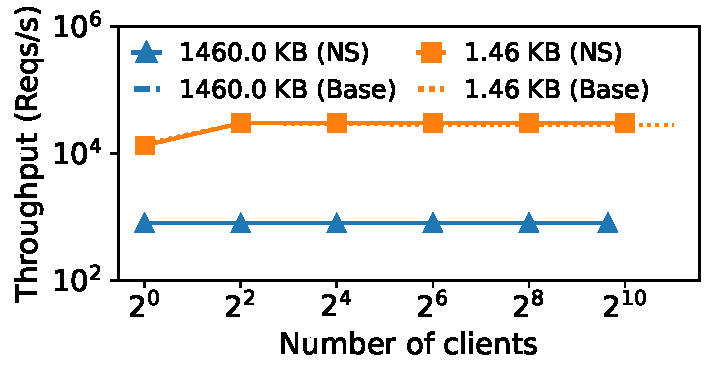
\includegraphics[width=\textwidth]{throughput_vs_client_num.pdf}
    \caption{\# clients vs throughput}
    \label{subfig:clients-vs-xput}
    \end{subfigure}
%    \hspace{30pt}
    \hfill
    \begin{subfigure}{0.49\columnwidth}
    \centering
    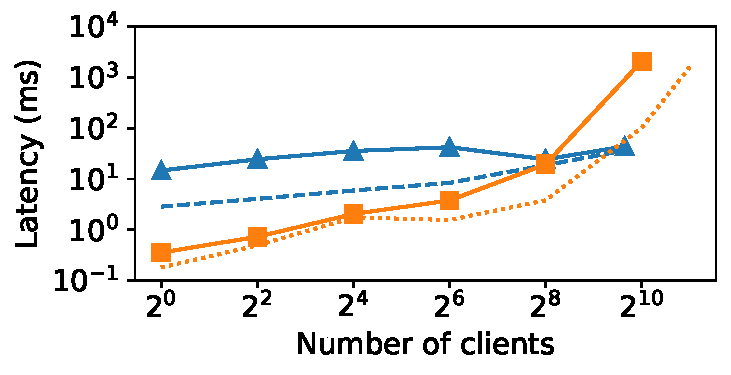
\includegraphics[width=\textwidth]{latencies_vs_client_num-logscale.pdf}
    \caption{\# clients vs latency}
    \label{subfig:clients-vs-latency}
    \end{subfigure}
    \caption{Throughput and latency overhead due to middleboxes without shaping.
%        \am{Show error bars.}
    }
    \vspace{-0.4cm}
    \label{fig:xput-latency-microbench}
\end{figure}

\textbf{Middlebox throughput.}
%We measure %the peak line rate,
%the peak throughput that can be sustained in a client-server system and the
%impact of concurrent clients on peak throughput and response latency.
\if 0
For line rate, we use iperf3 \citeme{iperf3} to generate a large number of
asynchronous requests from the client to the server and measure the peak load
sustained. \todo{We report the average line rate measured across three X min
runs of iperf3.} The {\base} sustains a line rate of \todo{9.4 Gbps} and, with
\todo{9.39 Gbps}, {\nsnoshape} can match the {\base} line rate. \am{Do we need
this?}
\fi
%
We measure the peak throughput (requests/s) attained by a server application,
the response latency experienced by the clients, and the impact on this
throughput and latency due to the middleboxes.
We restrict Nginx to one worker thread and one core on the server desktop.
We evaluate using two object sizes: 1.4 KB (one MTU) and 1.4 MB.
We identify the peak request rate that can be handled by a single wrk2 client,
then increase the clients until we find the peak throughput the server can
provide.
%Then, we vary the load by increasing the number of concurrent clients while
%fixing each client to generate the peak per-client request rate.
%Once we find the peak server throughput, we vary the number of
We then vary the number of concurrent clients while generating the peak request
load sustainable by the server to find the maximum number of concurrent clients
that the server can handle and to measure the impact on the response latency.

%For each object size, wrk2 generates a request load to the server for \update{3
%min}; we discard the measurements from the first minute to eliminate startup
%effects.
We run experiments for \update{3 min} and discard the measurements from the
first minute to eliminate startup effects.
\Cref{subfig:clients-vs-xput} shows the average of the peak throughput
observed across \update{3 runs}.
The standard deviation is \update{below 1\%} in all cases. For 1.4 KB and 1.4 MB
objects, the {\base} server achieves a peak throughput of \update{30K req/s}
\update(64 clients) and \update{800 req/s} (800 clients), respectively.
{\nsnoshape} matches the peak throughput and the max concurrent clients
sustained by {\base}.
%{\nsnoshape} achieves a peak throughput of \todo{29.3K req/s} and \todo{798
%req/s}, respectively.
%\todo{\Cref{tab:xput-nomask} shows the peak throughput averaged across 10 runs;
%the standard deviation is below 10\% in all cases.}
%\todo{{\nsnoshape} incurs at most \todo{5.3\%} overhead on the {\base} peak
%throughput.}
%\am{Combine directly with the experiment on \# of clients vs xput and latency?}

\if 0
\begin{table}[t]
    \centering
    \begin{tabular}{llll}
        \toprule
        \textbf{Component} & {Avg.} & {Std} & Max\\
        \midrule
        Baseline RTT & \todo{X} & \todo{X} & \todo{X}
        \\
        Shaped buffer prepare & \todo{X} & \todo{X} & \todo{X}
        \\
        {QUIC enqueue} & \todo{X} & \todo{X} & \todo{X}
        \\
        Receive path & \todo{X} & \todo{X} & \todo{X}
        \\
        Kernel overhead & \todo{X} & \todo{X} & \todo{X}
        \\
        \bottomrule
    \end{tabular}
    \caption{Breakdown of response latency (ms)}
    \label{tab:lat-breakdown}
\end{table}
\fi

\textbf{Latency.}
\Cref{subfig:clients-vs-latency} shows the average and standard deviation of
the response latencies over a \update{2 min} run.
%the \update{3 runs of 2 min}.
The ping latency between each pair of directly connected desktops is
\update{0.56 $\pm$ 0.18 ms.}
%With the small payload, the response latency until about 64 clients remains the
%same for {\base} and {\nsnoshape}, and with the large payload, {\nsnoshape}
%incurs upto \todo{30\%} overhead on the {\base} latency at peak throughput.
%
%We further breakdown the end-to-end latency for a single client to understand
%the overheads introduced by the middleboxes. Of the \todo{990 ms}, we can
%attribute \todo{420 ms} to the same path taken by a packet as in {\base}.
This overhead comes from the fact that
each packet traverses four additional network stacks (across two middleboxes) in
each direction. This also involves data copy operations between the kernel and
user space. The data copy overhead is proportional to the object size; thus
{\nsnoshape}'s latency overhead increases with the larger response sizes.
%\todo{\Cref{tab:lat-breakdown}} shows a breakdown of the latency between the
%time an application packet enters the middlebox and leaves over the tunnel.

The kernel data copy overheads are not fundamental to {\sys}'s design.
%
By using kernel bypass techniques or tools like DPDK \cite{dpdk}, {\sys} can
%eliminate data copies between user and kernel space and
reduce the latency overhead.
%By implementing {\sys} over DPDK \cite{dpdk}, which directly sends packets from
%userspace to the NIC, the overheads can be reduced.

\textbf{Shaping interval, preparation, and enqueue times.}
We further profile the middlebox execution to measure the max latencies of
the two components in the {\prepare} loop (\S\ref{sec:implementation}): the
preparation of the shaped buffer and queuing of the buffer to QUIC worker.
These measures determine the maximum
durations for preparing and
enqueueing shaped buffers ($\dpintvl_{prep}$ and $\dpintvl_{enq}$,
respectively), and the minimum value for the shaping interval
$\dpintvl$. We profile the delays with the middlebox configured
with \update{128 queues}, thus supporting a maximum of 128 concurrent clients.
%This implies that our middlebox can support a maximum
%of 128 concurrent clients.
One can profile the delays for a different
number of queues and concurrent clients.

Based on our measurements, we set \update{$\dpintvl_{prep} = 6 ms$ and
$\dpintvl_{enq} = 1 ms$}. The smallest
value for $\dpintvl$ that we can configure is \update{10ms}.
%$\dpintvl_{prep} = 7ms$, $\dpintvl_{enq} = 2ms$, and $\dpintvl = 10ms$.}
%Note that these are the smallest values required for the three
%parameters. In the next sections, we discuss the trade-off of choosing larger
%values, which increase latency overhead, but also reduce the privacy loss.

\textbf{Throughput and latency with shaping enabled.}
We now re-run the microbenchmarks with {\ns} configuration. We use three
different configurations for $\dpintvl$: \update{10ms, 50ms, and 100ms}.
%For each configuration, we measure the peak request rate sustained by the
%middlebox and the response latency observed by the clients at the peak
%throughput.
We use 128 concurrent clients. The middlebox can sustain the peak throughput of
\update{30K req/s with 1.4KB objects} and \update{700 req/s with 1.4MB} objects
for each configuration of $\dpintvl$. For 1.4KB objects, the average and standard
deviation of the response latency with the three configurations are as follows:
\update{(i) $\dpintvl = 10ms$: 30.47 $\pm$ 3.89 ms}, \update{(ii) $\dpintvl =
50ms$: 51.39 $\pm$ 14.64 ms, (iii) $\dpintvl = 100ms$: 77.49 $\pm$ 28.96 ms}.
For 1.4MB objects, the latencies are as follows:
\update{(i) $\dpintvl = 10ms$: 41.31 $\pm$ 10.84 ms}, \update{(ii) $\dpintvl =
50ms$: 76.96 $\pm$ 21.12 ms}, \update{(iii) $\dpintvl = 100ms$: 127.48 $\pm$
45.69 ms}.
%\am{why latencies in (ii) and (iii) are lower than loop interval?}
\update{The latency is dominated by the $\dpintvl$ configuration.}
The high variance in the latency is due to shaping.
%Requests may arrive at a middlebox at arbitrary times w.r.t. a decision loop
%interval.
If a request arrives just after the decision loop has prepared a buffer in the
current iteration, the request will be delayed by at least one iteration of the
loop.
Moreover, a negative sampling of DP noise may lead to a smaller shaped buffer
than the available payload bytes in the buffering queues, thus delaying the
requests by one or more intervals. This effect is particularly enhanced in a
workload close to the line rate. Thus, {\sys} can perform well within about 12-15\%
of the line rate.

\textbf{CPU utilization.}
\update{The CPU utilization is 3-10\% for the {\prepare} core and depends on the
DP shaping interval; the utilization is 8-70\% for the QUIC worker core,
which depends on the network I/O. The {\ushaper} core utilizes 100\% of the CPU as
it polls for packets from {\prepare}. As such, the {\prepare} and QUIC worker
cores would be able to support additional tunnel instances by time-sharing their
core. By using a polling
interval, we could reduce the CPU utilization of {\ushaper} to support
additional requests at the cost of additional latency.
In general, multiple tunnels can time-share the same physical cores, as long as
each core runs the same type of thread, to suffice property P4 mentioned in
\S\ref{sec:implementation}.
}


\subsection{Case Study: Video Streaming}
\label{subsec:eval-video}

\begin{figure}[t]
  \centering
  \begin{subfigure}{0.49\columnwidth}
      \centering
%
%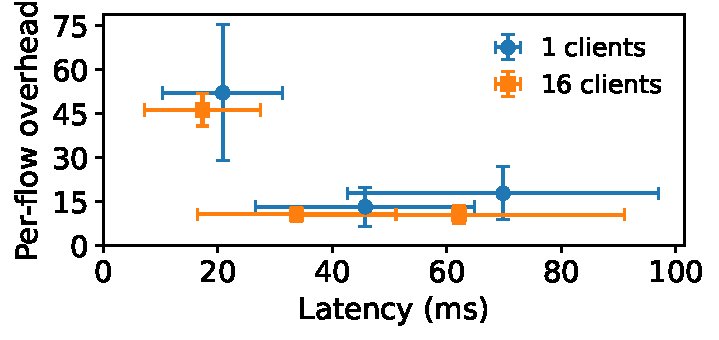
\includegraphics[width=\textwidth]{plots/bw_overhead_vs_latencies_web.pdf}
      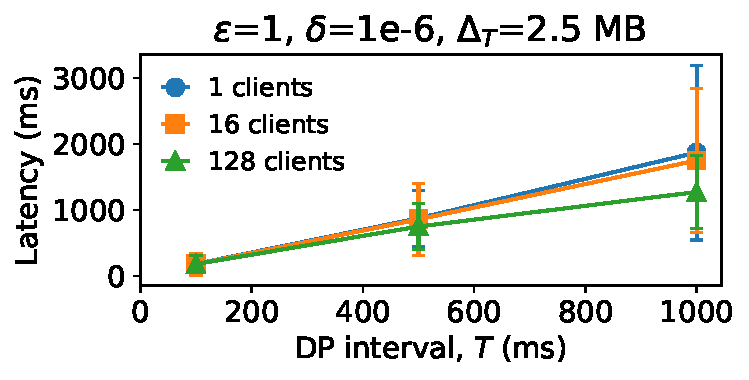
\includegraphics[width=\textwidth]{latency_vs_dp_interval_video_updated.pdf}
      \caption{Latency vs DP interval}
      \label{fig:video-lat-vs-dpInt}
  \end{subfigure}
  \hfill
  \begin{subfigure}{0.49\columnwidth}
      \centering
      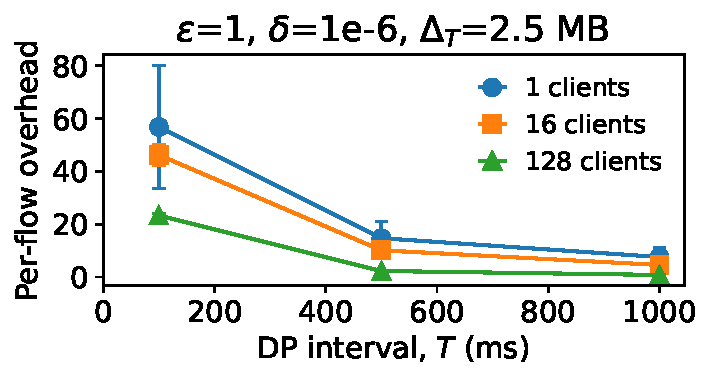
\includegraphics[width=\textwidth]{overhead_vs_dp_interval_video_updated.pdf}
      \caption{BW overhead vs DP interval}
      \label{fig:video-overhead-vs-dpInt}
  \end{subfigure}
  \begin{subfigure}{0.49\columnwidth}
      \centering
      %
      %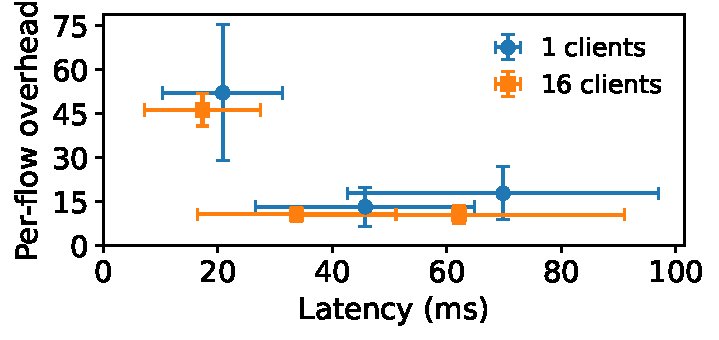
\includegraphics[width=\textwidth]{plots/bw_overhead_vs_latencies_web.pdf}
      \includegraphics[width=\textwidth]{latency_vs_dp_interval_web_updated.pdf}
      \caption{Latency vs DP interval}
      \label{fig:web-lat-vs-dpInt}
  \end{subfigure}
  \hfill
  \begin{subfigure}{0.49\columnwidth}
      \centering
      \includegraphics[width=\textwidth]{overhead_vs_dp_interval_web_updated.pdf}
      \caption{BW overhead vs DP interval}
      \label{fig:web-overhead-vs-dpInt}
  \end{subfigure}
  \caption{Latency and bandwidth overhead for different
  values of DP interval for video streaming (a, b) and for web (c, d).\\}
  \begin{subfigure}{0.485\columnwidth}
      \centering
      %
      %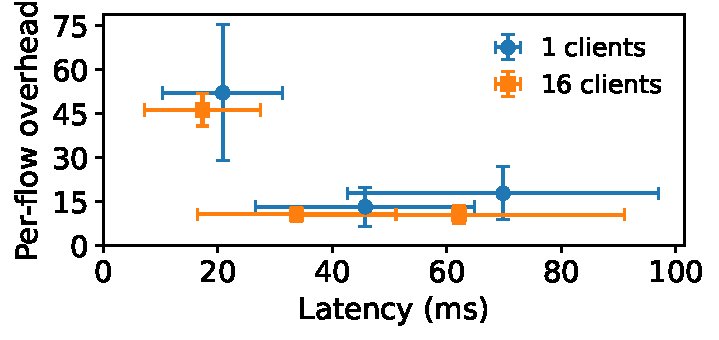
\includegraphics[width=\textwidth]{plots/bw_overhead_vs_latencies_web.pdf}
      \includegraphics[width=\textwidth]{overhead_vs_number_of_traces_video_bidirectional_loglog_updated.pdf}
      \caption{Video streaming.}
      \label{fig:video-overheads-compare}
  \end{subfigure}
  \hfill
  \begin{subfigure}{0.49\columnwidth}
      \centering
      \includegraphics[width=\textwidth]{overhead_vs_number_of_traces_web_bidirectional_loglog_updated.pdf}
      \caption{Web service.}
      \label{fig:web-overheads-compare}
  \end{subfigure}
  \caption{Comparison of {\sys}, constant shaping, Pacer.}
  \vspace{-0.4cm}
\end{figure}
Next, we examine the effect of different privacy settings on bandwidth and
latency overheads for video streaming clients.

%\textbf{Latency vs bandwidth overhead.}
%We configure the DP shaping interval $\dpintvl$ in the middleboxes and
%measure
%the response latencies for individual video segments with the testbed. For the
%same $\dpintvl$ and for a fixed $\ssens$ and $\varepsilon_{\winlen}$, we measure
%the bandwidth overhead for the video streams in the simulator.
We run experiments with three values of $\dpintvl$
for the server: 100ms, 500ms, and 1s, and max per-flow DP length cutoff of
1.21 MB, 1.22MB, and 1.7 MB, respectively. We use
\update{$\qsens = 2.5 MB$} and
\update{$\varepsilon = 1$}.
For all experiments, we set the DP parameters for client request traffic as
follows: \update{$\qsens = 200$}~bytes, $\winlen = 1s$, $\dpintvl = 10ms$,
\update{$\varepsilon = 1$} and max per-flow DP length cutoff of 206 bytes.
We run experiments with 1, 16, and 128 video
clients; each client requests one video randomly selected from the dataset.
For each set of configurations, we measure the average response latency for
individual video segments with the testbed as well as the per-flow relative
bandwidth overhead for the video streams in the simulator.

\textbf{Latency and bandwidth overhead.}
%For each value of $\dpintvl$, we vary video clients between 1 to 16, with each
%client streaming one video randomly selected from the dataset.
%In \update{\Cref{fig:video-lat-vs-xput}},
%the x axis shows the
%%\todo{average and standard deviation} of
%the download latency across all video segments.
%The y axis shows the
%%\todo{average and standard deviation of the per-flow}
%\update{average per-flow}
%relative bandwidth overhead across all videos streamed
%by the concurrent clients.
\Cref{fig:video-lat-vs-dpInt,fig:video-overhead-vs-dpInt} respectively show the
average segment download latency and the average per-flow relative bandwidth
overhead as a function of different intervals and for varying number of clients.
The {\base} segment download latency is \update{2.86 $\pm$ 1.41ms.} The latency
variance is due to variances in the segment sizes.
The relative bandwidth overhead of a video is the
number of dummy bytes transmitted normalized to the size of the unshaped video
stream.
The error bars show the standard deviation in latency and bandwidth overhead.

First, \Cref{fig:video-lat-vs-dpInt} shows that, for all values of $\dpintvl$,
the video segments can be downloaded well within 5s, which is the time to play
each segment and request the next segment from the server.
\update{The high variance is due to negative DP noise, which delays
payload transmission.}
Secondly, the results show the trade-off between latency and bandwidth. A larger
DP interval implies higher download latency but fewer queries, thus
yielding a lower bandwidth overhead.
%Moreover, $\dpintvl = 2.5s$ incurs a total bandwidth overhead of \todo{X MB} for
%a single client.
Thirdly, with multiple concurrent clients, the bandwidth overhead is
amortized, while the average download latency only depends on $\dpintvl$.
Overall, {\sys} can secure video streams with low bandwidth overheads
and no impact on the streaming experience.


\subsection{Case Study: Web Service}\label{subsec:eval-web}
%We analyze the overheads on bandwidth, client response
%latency, and peak server throughput of a web service.
%\begin{figure}[t]
%  \centering
%  \begin{subfigure}{0.49\columnwidth}
%      \centering
%%
%%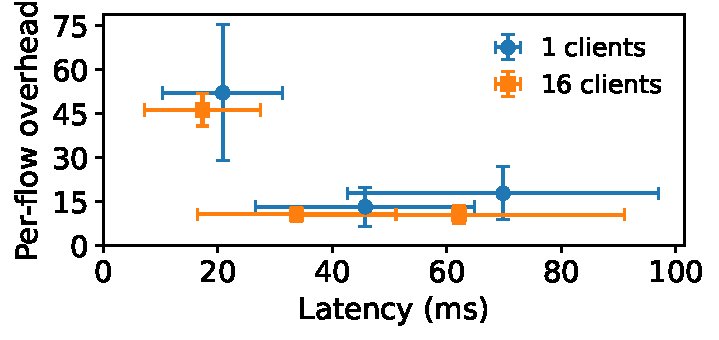
\includegraphics[width=\textwidth]{plots/bw_overhead_vs_latencies_web.pdf}
%
%\includegraphics[width=\textwidth]{plots/latency_vs_dp_interval_web_updated.pdf}
%      \caption{Latency vs DP interval}
%      \label{fig:web-lat-vs-dpInt}
%  \end{subfigure}
%  \hfill
%  \begin{subfigure}{0.49\columnwidth}
%      \centering
%
%\includegraphics[width=\textwidth]{plots/overhead_vs_dp_interval_web_updated.pdf}
%      \caption{BW overhead vs DP interval}
%      \label{fig:web-overhead-vs-dpInt}
%  \end{subfigure}
%  \caption{\update{Web service. Latency and bandwidth overhead for different
%  values of DP interval.}
%  }
%\end{figure}
We perform similar experiments as \S\ref{subsec:eval-video} with our web
service. For the server responses, we use \update{$\qsens = 60 KB$}, $\winlen =
1s$, and \update{$\varepsilon = 1$}. We use $\dpintvl$ of {10ms, 50ms, and
100ms}, and per-flow DP length cutoffs of 60.8KB, 60.8KB, and 110.9KB,
respectively.
For the client requests, we use the same configs as in
\S\ref{subsec:eval-video}. We run \update{3 min} experiments with 1, 16, and 128
wrk2 clients with a total load of \update{1600 req/s};
each client requests random web pages from the dataset. We discard the numbers
of the first minute.

\textbf{Latency and bandwidth overhead.}
%For each value of $\dpintvl$, we vary wrk2 clients between 1 to 16, with each
%client requesting several web pages randomly selected from the dataset.
%\update{\Cref{fig:web-lat-vs-xput}} presents the average response latency versus
%the \update{average per-flow} relative bandwidth overhead across all
%requested pages. The error bars indicate standard deviation.
%
%The figure shows that {\sys} can sustain peak throughput in all configurations.
\Cref{fig:web-lat-vs-dpInt,fig:web-overhead-vs-dpInt} respectively show the
average response latency and the average per-web page relative bandwidth
overhead, across all web page requests.
The {\base} latency is \update{0.225 $\pm$ 0.3 ms}. (The high variance is due to
the time precision in wrk2 being restricted to 1ms.)
%{\ns} latency at peak throughput is $\todo{X} ms$, $\todo{X} ms$, and $\todo{X}
%ms$ with $\dpintvl$ of \todo{0.01ms}, \todo{0.05ms}, and \todo{0.1ms},
%respectively.
The web workload is more sporadic than video streaming, thus web page download
latencies have higher variance than video segment download latency.
The absolute latency overhead for {\ns} depends on the choice of $\dpintvl$. The
relative overhead depends on the underlying network latency, which unlike our
testbed, is in the order of 10s to 100s of milliseconds in the Internet.
%
%The web traffic is much smaller than video streams. Hence, for
%similar privacy loss and number of DP queries, the bandwidth overhead is
%higher for the smaller web traffic.
Interestingly, the bandwidth overhead for web traffic first reduces with
increasing DP shaping interval from 10ms to 50ms, but then increases again
with an interval of 100ms. This is because, for small web pages, the DP interval
of 100ms is larger than the total time required to download web pages. As a
result, additional overhead is incurred due to the padding of traffic in the
100ms intervals.

\subsection{Comparison with other techniques}\label{subsec:eval-comparison}
%\begin{figure}[t]
%  \centering
%  \begin{subfigure}{0.49\columnwidth}
%  \centering
%%
%%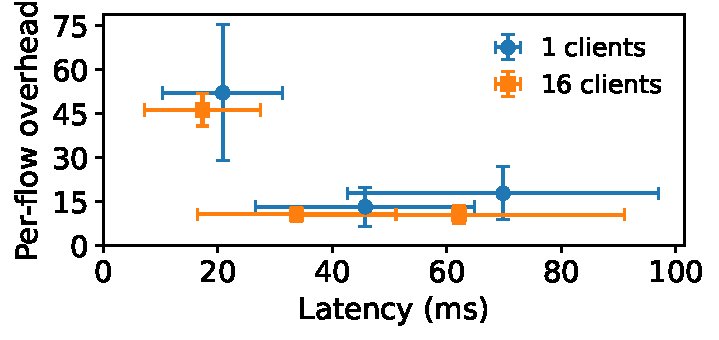
\includegraphics[width=\textwidth]{plots/bw_overhead_vs_latencies_web.pdf}
%
%\includegraphics[width=\textwidth]{plots/overhead_vs_number_of_traces_video_bidirectional_loglog_updated.pdf}
%      \caption{Video streaming.}
%      \label{fig:video-overheads-compare}
%  \end{subfigure}
%  \hfill
%  \begin{subfigure}{0.49\columnwidth}
%      \centering
%
%\includegraphics[width=\textwidth]{plots/overhead_vs_number_of_traces_web_bidirectional_loglog_updated.pdf}
%      \caption{Web service.}
%      \label{fig:web-overheads-compare}
%  \end{subfigure}
%  \caption{\update{Comparison of {\sys}, constant shaping, Pacer.}
%  }
%\end{figure}

%\textbf{Comparison with other techniques.}
\Cref{fig:video-overheads-compare,fig:web-overheads-compare} show the per-flow
relative bandwidth overhead of {\ns},
%(different $\varepsilon$ values),
{\constshape}, and {\pacer} for video and web
applications, respectively, for varying number of concurrent flows.
%We compare overhead of {\ns} with constant rate shaping ({\constshape})
%and~Pacer \cite{mehta2022pacer}.

% For {\constshape}, we configure the peak load for video service corresponding to
% transmitting 1.7MB in every 5s, and the peak load for web service corresponding
% to transmitting 57KB every 50ms. These rates correspond to transmitting at a
% rate that covers the largest object sizes in our video and web datasets.

% In Pacer, for video service, we pad a segment at $i$\textsuperscript{th} index
% in a video stream to the largest segment size at that index across all videos in
% the dataset. For web service, we pad all web pages to the largest page size,
% \ie 147KB in our dataset.

For both video and web traffic, {\ns} incurs three orders of magnitude lower
overhead than {\constshape}, which requires continuously transmitting traffic at
the peak server load (configured for 1000 clients).
%
%For video traffic, {\ns} requires 11 flows to achieve lower overhead than
%{\pacer}.
%For video traffic, while {\ns} incurs similar overhead as Pacer for a single
%flow with \update{$\varepsilon = 1$}, it can further amortize its overheads
%among multiple concurrent streams within the tunnel without compromising
%privacy.
%Specifically, the per-stream overheads become lower than those of
%%{\constshape} and
%Pacer with just \todo{5} streams and are \todo{$ <10\%$} with \todo{10}
%streams.
%\am{It might look like we cherrypicked Pacer for comparison. Maybe
    %Pacer comparison can go.}
%Unlike {\constshape} and Pacer, {\ns} can amortize overheads among
%multiple concurrent streams sharing the same tunnel without compromising
%privacy.
%\Cref{fig:video-overheads-compare} illustrate per-flow bandwidth overhead of
%{\ns} with different values of privacy loss compared to other methods. We use
%an update interval of 1 s, sensitivity of 1 MB, and measure the per-flow
%overhead and privacy loss of segments of 5 s respectively.
%Note that unlike other methods such as Pacer \cite{mehta2022pacer} and constant
%rate shaping, the bandwidth overhead of {\sys} depends on the number of parallel
%flows going through our middlebox.
%Specifically, when a channel of information between two middleboxes became
%differentially private, all flows going through the channel leverage the same
%level of privacy.
%Therefore, the per flow overhead decreases based on the number of flows. For
%example, with about 100 parallel streams going through {\sys} middlebox, the
%per-stream overhead is as small as 10\% of the actual size of streams.
%
%\textbf{Comparison with other techniques.}
%\Cref{fig:web-overheads-compare} shows the relative bandwidth overhead, per web
%request, varying with number of concurrent requests and for different values of
%$\varepsilon_{\winlen}$. Again, the overhead of {\ns} is three orders of
%magnitude lower than that of {\constshape}.
%%Here, {\ns} incurs higher overheads than Pacer,
%For web traffic, {\ns} requires more than \update{40 flows}
%%\update{20 flows at $\varepsilon_{\winlen} =
%%16$} and \update{60 flows at $\varepsilon_{\winlen} = 4$}
%to achieve lower overhead than {\pacer}.
For video and web traffic, {\ns} requires 11 flows and more than 40 flows,
respectively to achieve lower overhead {\pacer}.
Pacer shapes server traffic only upon receiving a client request and does not
shape client traffic. Thus, it leaks the timing and shape of client requests,
which could potentially reveal information about the server responses
\cite{chen2010reality}.
{\sys} shapes traffic in both directions, which incurs higher overhead at the
cost of stronger privacy than Pacer.
%\todo{Explain.}
%Moreover Pacer pads the server response to the largest page length
%in the server's dataset and stops transmitting after a number of packets
%corresponding to the largest page length have been transmitted.
%\todo{In contrast, {\sys} continuously shapes traffic for 1s windows.}
%\am{Need to make this more precise}.





\if 0
\paragraph{Bandwidth overhead vs privacy loss.}
We compare the bandwidth overhead for web traffic due to {\ns}, {\constshape},
and Pacer in \Cref{fig:web-overheads-compare}.
\todo{We use $\winlen = 1 s$, $\dpintvl = 0.1 s$, $\ssens = 150 KB$, and the
same values of $\varepsilon_{\winlen}$ as in \S\ref{subsec:eval-video}, and we
measure the per-flow overhead until each web page is downloaded.}

\todo{Here, {\ns} incurs higher overheads than Pacer because Pacer only pads all
web pages to the largest page length in a service's dataset, whereas {\ns}
performs traffic shaping without any prior knowledge of the page sizes.} \am{Not
convinced about the argument here. $\ssens$ is chosen somewhat based on the
dataset; the overheads would vary based on $\ssens$.}
%We use the same metric of \Cref{subsec:eval-video} to measure the bandwidth
%overhead of {\sys} in shaping traffic of web services with different levels of
%privacy loss. With an update interval of 100 ms and sensitivity of 150 KB, we
%measure the per-flow overhead of {\sys} shaping mechanism and aggregated
%privacy loss for windows of 1 second.

%It is worth noting that the overhead of Pacer \cite{mehta2022pacer} is notably
%low, as it pads all webpages to their maximum size prior to transmission.
%In contrast, {\sys} performs traffic shaping without any prior knowledge of the
%page sizes.
\fi

\smallskip\noindent
\textbf{Evaluation summary.}
{
Our evaluation provides four insights.
(i) There is a huge gap between the theoretical DP guarantees and the
privacy configurations required to defeat SOTA attacks.
%Theoretical analysis suggests that you need quite strong privacy guarantees, but
%from a practical perspective, applications require much weaker guarantees.
%(ii) the costs of privacy required in the face of more sophisticated attacks in
%the future,
(ii) The latency overhead is dominated by the choice of DP shaping interval,
(iii) {\sys}'s middlebox can match about 88\% of the 10Gbps NIC line rate; a
single core of
{\ushaper} can match the peak throughput of a single core server,
(iv) {\sys}'s cost is in the two additional cores for {\prepare} and QUIC worker,
which helps to avoid any secret-dependent interference in shaping and keep low DP
shaping loop lengths. By optimising the implementation, we could use a
single middlebox to support larger workloads.
%The CPU utilization is 3-10\% for the {\prepare} core and depends on the loop
%interval; the utilization is 8-70\% for the QUIC worker core, which depends on
%network I/O. The {\ushaper} core utilizes 100\% of the CPU as it polls for
%packets from {\prepare}. As such, the {\prepare} and QUIC worker cores would be
%able to support additional application cores. By using a polling interval, we
%could reduce the CPU utilization of {\ushaper} to support additional requests at
%the cost of additional latency.
%\am{provide an estimate of scaling the cores.}
%negligible compared to the overheads due to DP shaping.
}
